% -< SECTION
% >--------------------------------------------------------------------
\section{Evaluation}\label{sec:evaluation}
We validate our LISP/LISP-MN implementation by conducting a simulation \ed{BD:
it is unclear to me how, at 1st glance, running a simulation can validate a
simulator (while you mention that in the Introduction)?} and providing a
preliminary performance evaluation of handover delay.
The topology used for the simulation is shown in Fig.~\ref{sim_scenario}.
\ed{BD: you could redraw this figure so that text appears larger}

%-< FIGURE >--------------------------------------------------------------------
\begin{figure}[!th]
	\centering
	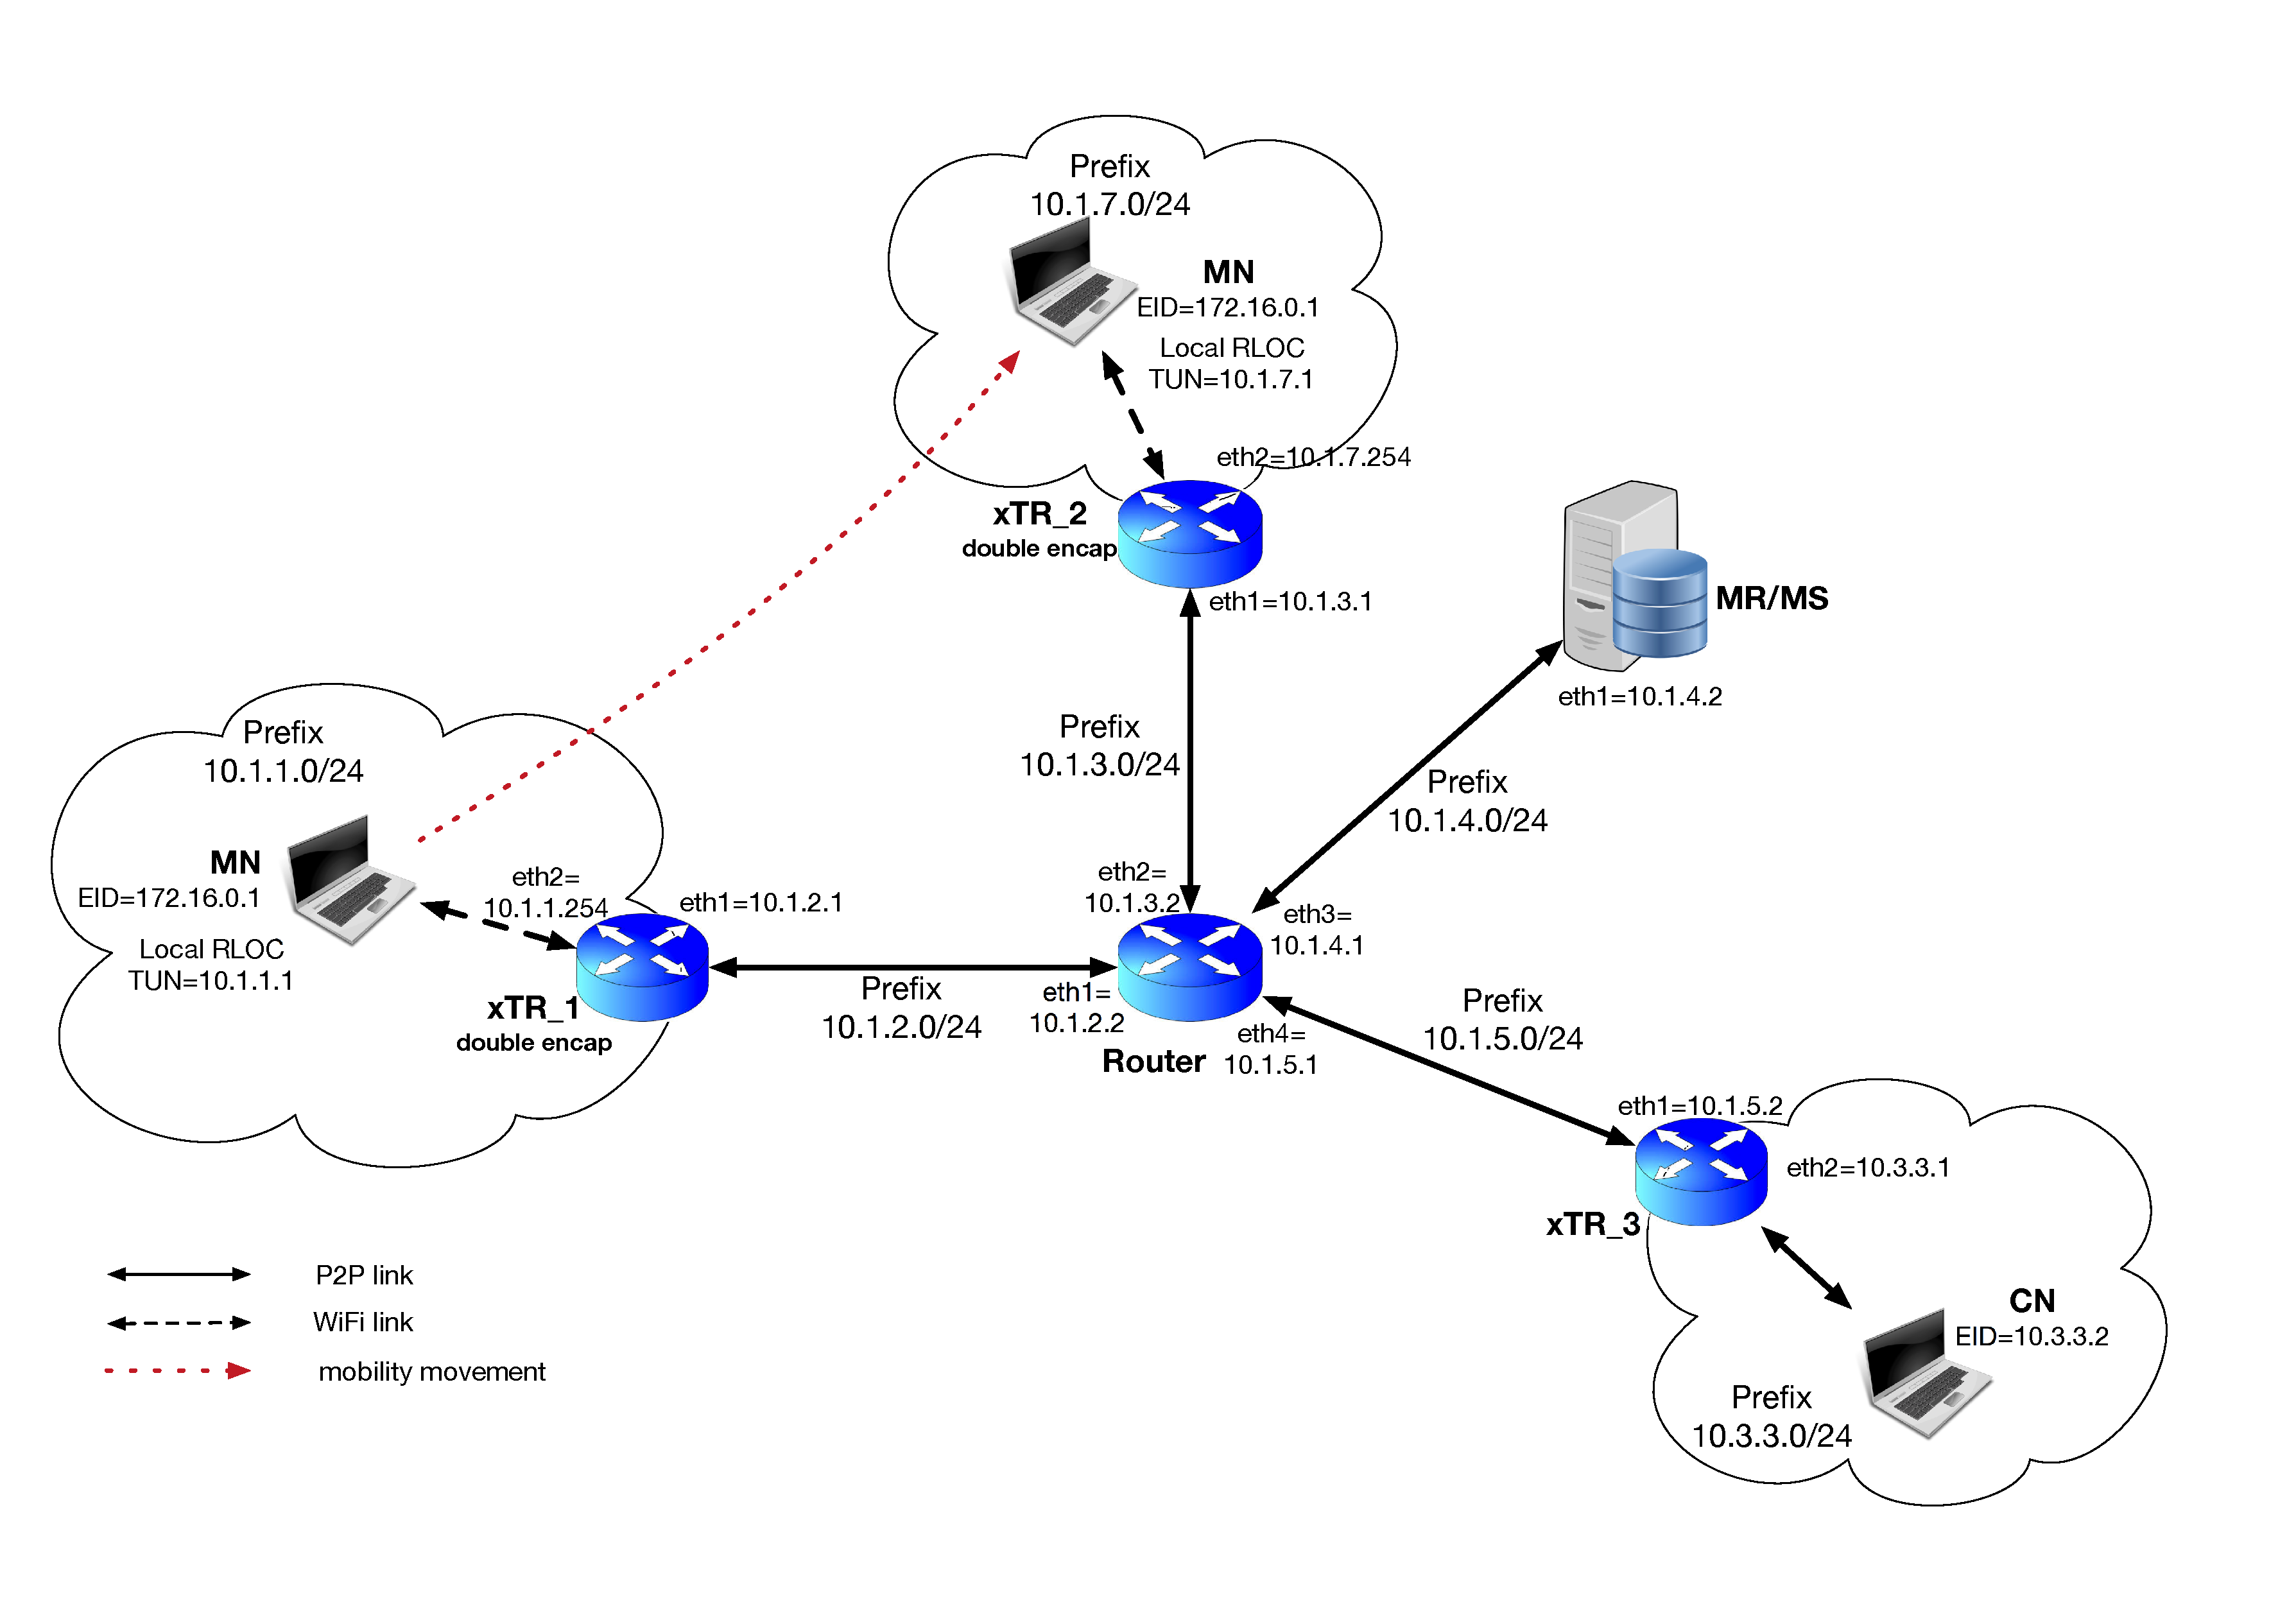
\includegraphics[width=0.5\textwidth]{Pics/mobility_through_subnets_2_encap_topo}
	\caption{LISP mobility simulation scenario for double encapsulation}
	\label{sim_scenario}
\end{figure}
%-< END FIGURE >--------------------------------------------------------------------

% -< SUB SECTION
% >--------------------------------------------------------------------
\subsection{Simulation Setup}\label{sec:setup}
In our simulation, a LISP-MN with permanent EID 172.16.0.1 is initially placed
in network 10.1.1.0/24. An \emph{echo} application on LISP-MN sends one packet
per second to a remote stationary node CN with EID 10.3.3.2, and the LISP-MN
moves into network 10.1.7.0/24 at speed of $7.07m/s$ \ed{BD: why that speed?}.
The distance between xTR\_1 and xTR\_2 is $170m$. LISP-MN node uses Wi-Fi to
connect to xTR\_1. At a certain moment during the move, the Wi-Fi link between
LISP-MN and xTR\_1 goes down, triggering so the handover procedure. Afterwards,
LISP-MN connects to xTR\_2 and reestablishes the communication with CN node. The
total simulation time is set to $45s$ and the DHCP procedure delay is set to
$1s$. We conduct many times of simulations \ed{BD: how many?  Did you average
the results?  If so, what is your confidence in the average (i.e., you
have to compute for each average the confidence interval)?} with the various
beacon interval of Wi-Fi channel in the range of $0.05s$ to $2s$ \ed{BD: why?}.


% -< SUB SECTION
% >--------------------------------------------------------------------
\subsection{Results}\label{sec:results}
As shown in Fig.~\ref{sim_schema}, when MN sends the packets to CN during the
simulation, it needs double encapsulation and the packet flow sequences are as
follows. The traditional IP packets with EID 172.16.0.1 as source address and
EID 10.3.3.2 as destination address are encapsulated by adding Local RLOC
10.1.1.1 as outer source address and RLOC 10.1.5.2 as outer destination address
after MN querying the mapping information to MR. The LISP packets are
encapsulated and forwarded to xTR\_1. The latter gets the mapping information
from MR and encapsulates the packets again by adding the RLOC 10.1.2.1 as the
outer source address and RLOC 10.1.5.2 as the outer destination address, then
sends the packets on Internet core. The xTR\_3 needs decapsulate the packets
twice after it receiving and verifying the packets, and finally sends to CN.
Once LISP-MN lost its Wi-Fi connection with xTR\_1, it needs a DHCP procedure
(consisting of DHCP Discover, DHCP Offer, DHCP Request and DHCP ACK) with xTR\_2
to get a new LRLOC 10.1.7.1 and then triggers LISP SMR to xTR\_3. After xTR\_3
getting new mapping information of <10.1.7.1, 10.1.3.1> and <172.16.0.1,
10.1.7.1>, the connection between LISP-MN and CN is re-established again.

%-< FIGURE >--------------------------------------------------------------------
\begin{figure}[!th]
	\centering
	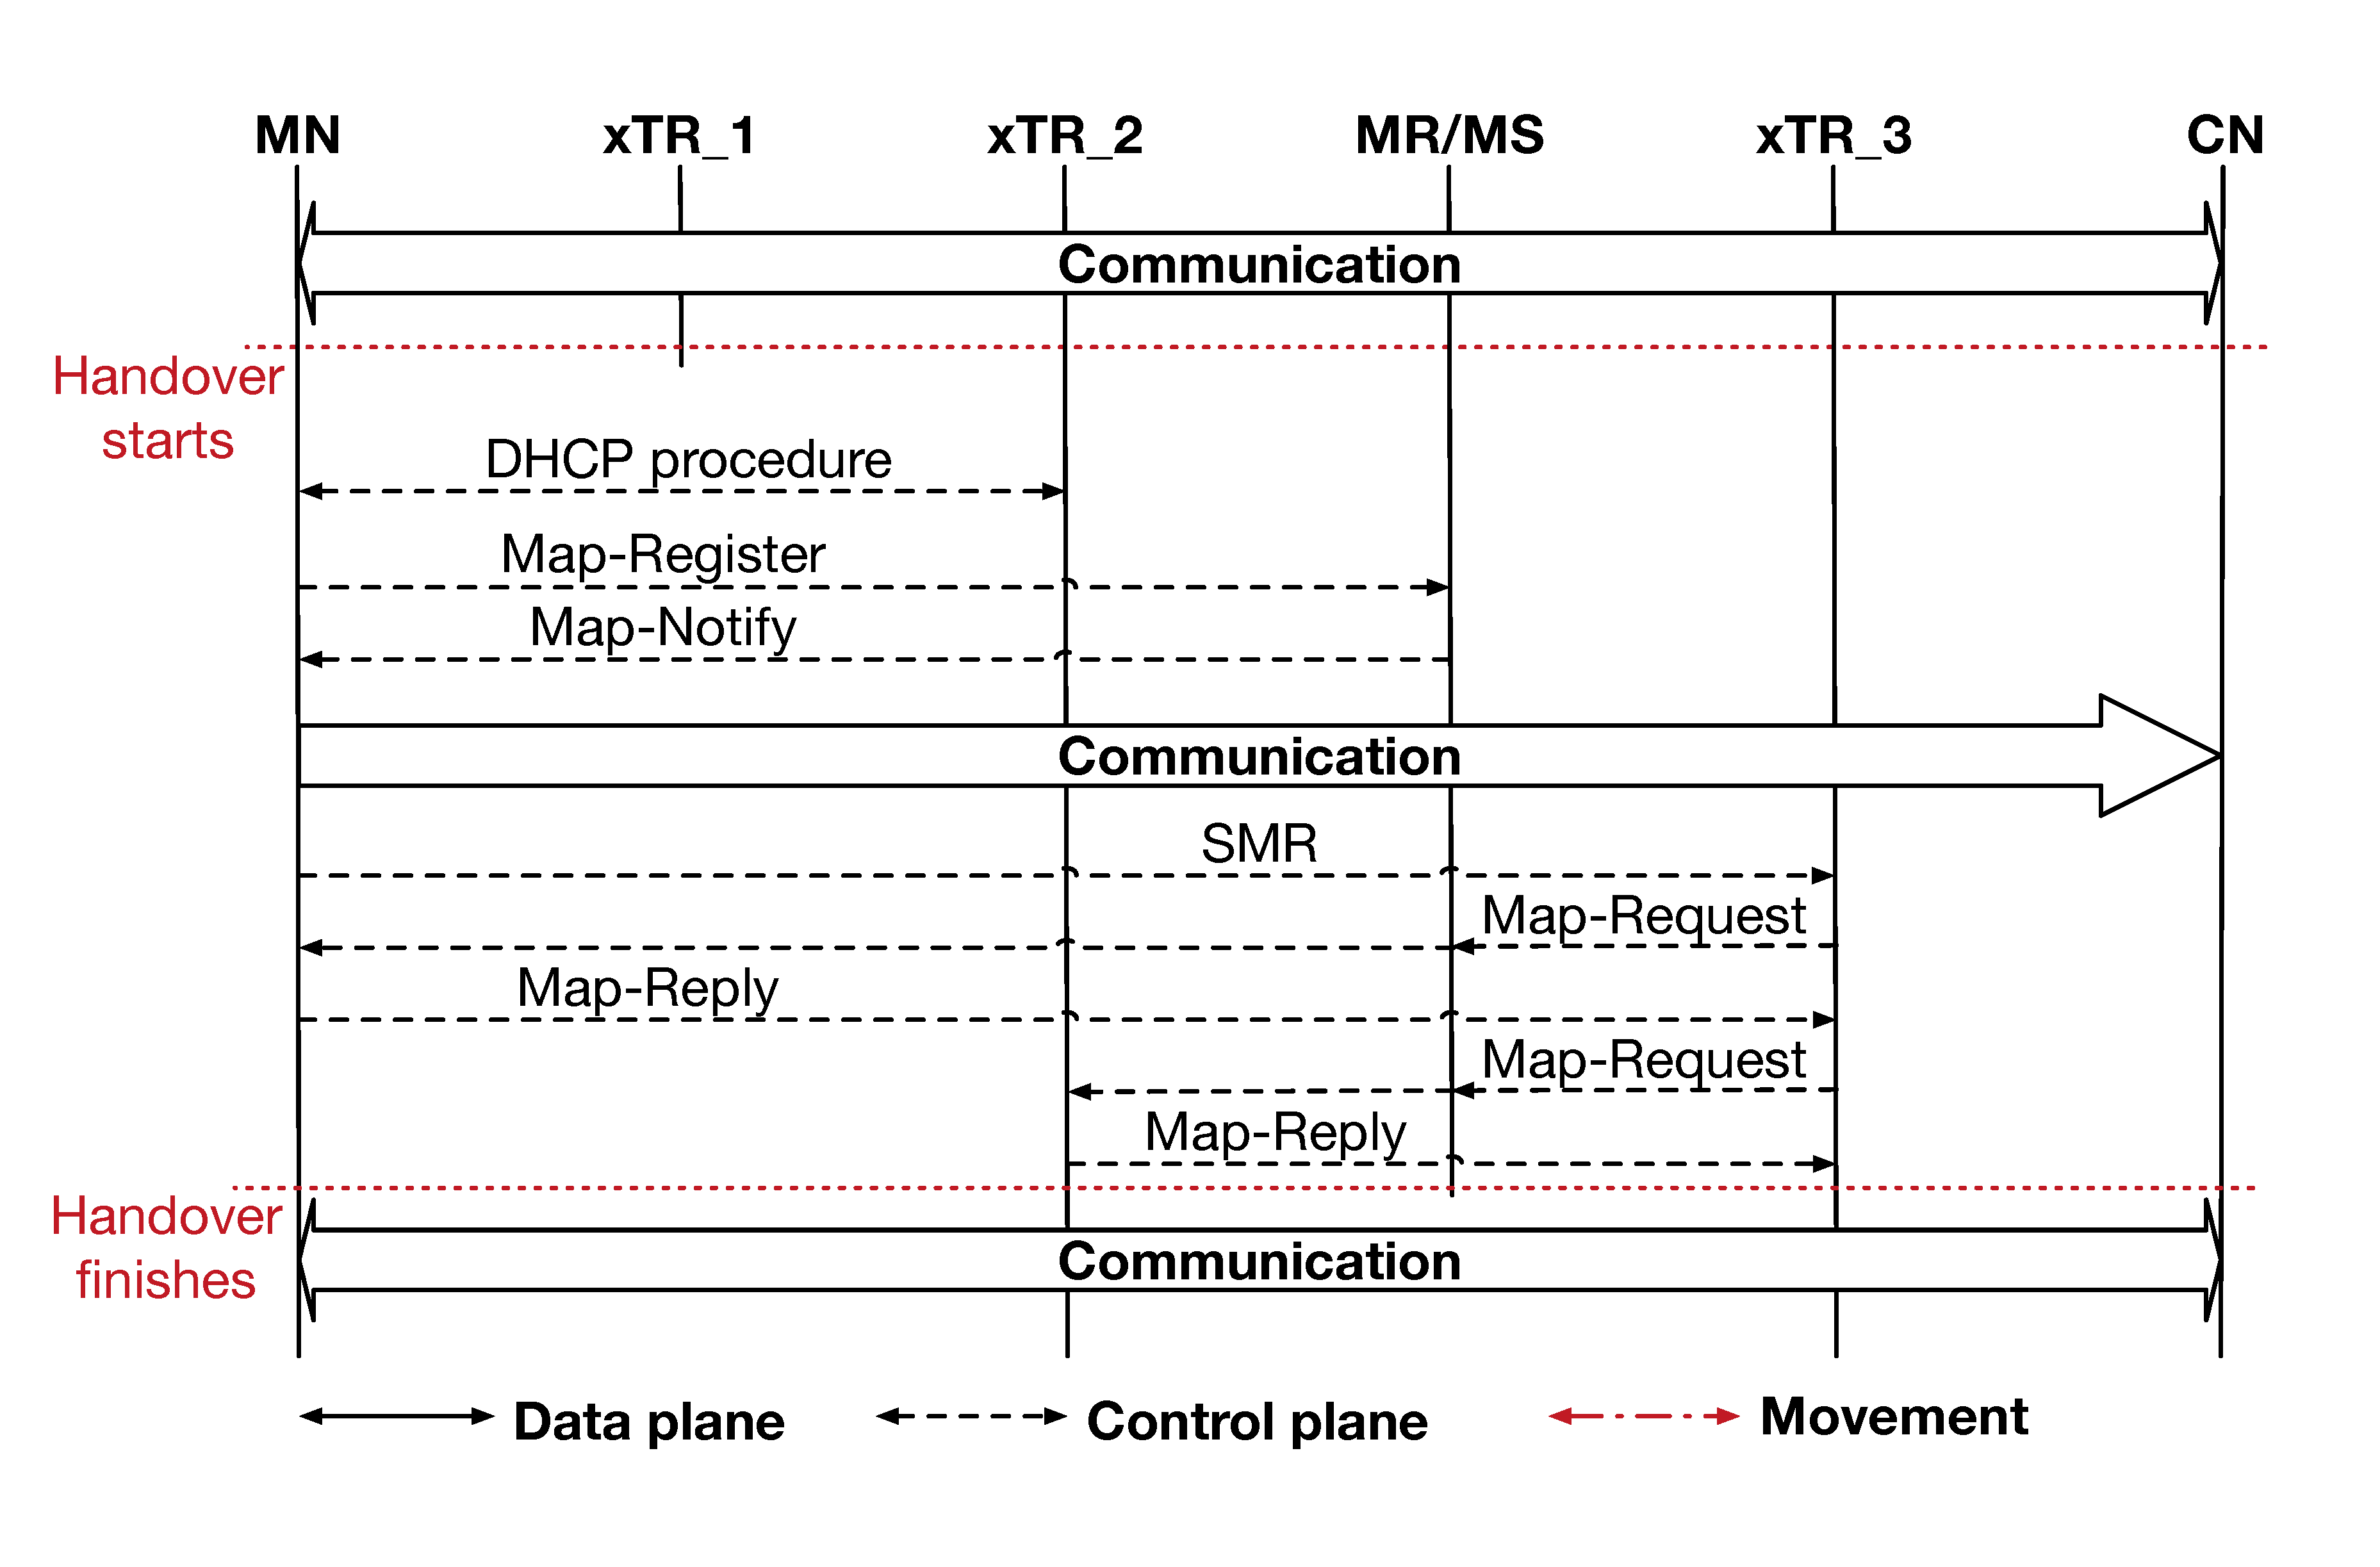
\includegraphics[width=0.5\textwidth]{Pics/Mobility_router_MN_supports_LISP_schema_SMR_simplify}
	\caption{Schema for LISP-MN mobility}
	\label{sim_schema}
\end{figure}
%-< END FIGURE >--------------------------------------------------------------------

The overall handover delay in this paper is defined at the moment that LISP-MN
sending DHCP Discover message to xTR\_2 and end up with xTR\_3 receiving the
last Map-Reply from xTR\_2 \ed{BD: unclear}. Precisely, it is made of three
parts:
the Wi-Fi association delay, the DHCP related delay, and LISP SMR delay:
\begin{equation}
    D_{overall} = D_{Wi-Fi}(BI) + D_{DHCP} + D_{SMR} \nonumber .
\end{equation}
where $D$ is the delay, $BI$ is Beacon Interval, subscriptions $Wi-Fi$, $DHCP$
and $SMR$ respectively refers to Wi-Fi association, DHCP procedure and LISP SMR.

After several runs \ed{BD: How much?} of the simulation, we observe
that the overall handover delay changes by the various beacon intervals, in particular the Wi-Fi
association delay depends on the different beacon intervals, whereas LISP SMR
procedure always cost around $3s$. To get the lower bound of overall handover
delay, we can ignore the Wi-Fi association delay when the beacon interval is
$500ms$, and the latency due to DHCP procedure is always $1s$. Thus, adopting
LISP-MN to conduct the host-based mobility takes at least $4s$. Compared to
current most stable solution for host-based IP mobility management MIPv6, which
latency including L2 and L3 in a real Wi-Fi testbed is around
$3.68s$~\cite{vassiliou2010analysis}, LISP-MN has a higher delay caused by the
double encapsulation mechanism introduced by LISP-MN behind LISP-Site.

During handover, CN can successfully receive packets from LISP-MN right after
DHCP procedure being accomplished, but LISP-MN cannot receive the packets from
CN until LISP SMR procedure is also finished. Thus, during DHCP procedure, all
bi-directional transmitted packets are lost. To improve the performance,
\cite{tang2017lisp} proposes a network-level LISP-MN solution, but has not
validated their proposals neither in simulation nor in testbed. Our ns-3
implementation can be used to realize them.

\ed{BD: I'm a little bit puzzled here.  I'm not sure what you really evaluate
in the sense that you rather provide a description of what happens during each
simulation run (i.e., message flow).  Do you have some quantification results
(for instance the latency variation over something)?}
